\section{Deployment at Volc\'{a}n Tungurahua}
\label{sec-deploy}

To demonstrate the value of wireless sensor networks for volcanic
monitoring, we deployed a small infrasonic monitoring network,
using the design in the previous section, at
Volc\'{a}n Tungurahua, an active volcano in central Ecuador.
Our network consisted of three infrasonic monitoring nodes, 
continuously transmitting infrasonic signals at 102~Hz to a central 
aggregator node, which relayed the data over a wireless link to an
observatory approximately 9~km from the monitoring station.
The deployment was active from July 20--22, 2004 and collected over
54~hours of infrasonic signals. During this time, the volcano was
erupting at the rate of several small or moderate explosions an hour.

\begin{figure}[t]
\begin{center}
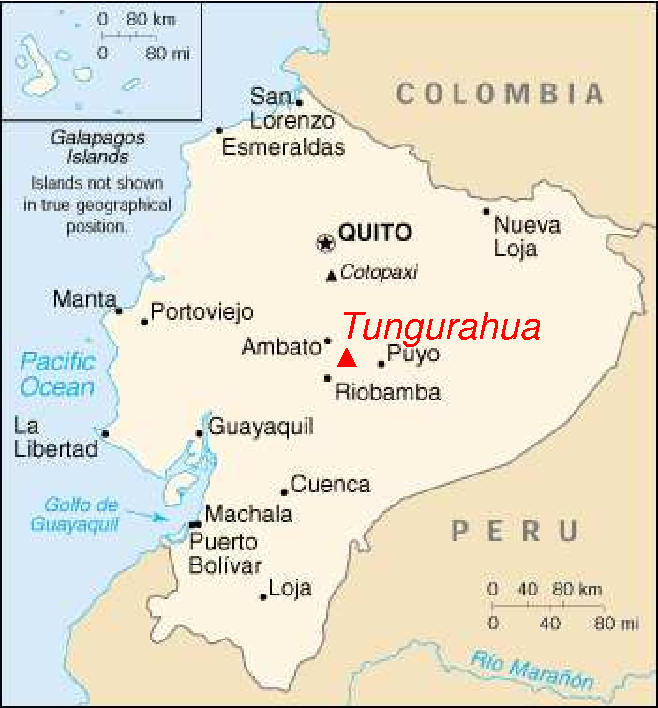
\includegraphics[width=0.7\hsize]{./figures/tungurahua.pdf}
\end{center}
\caption{\small {\bf Map showing location of Volc\'{a}n Tungurahua.}}
\label{fig-map}
\end{figure}

\subsection{Volc\'{a}n Tungurahua}

\begin{figure}[t]
\begin{center}
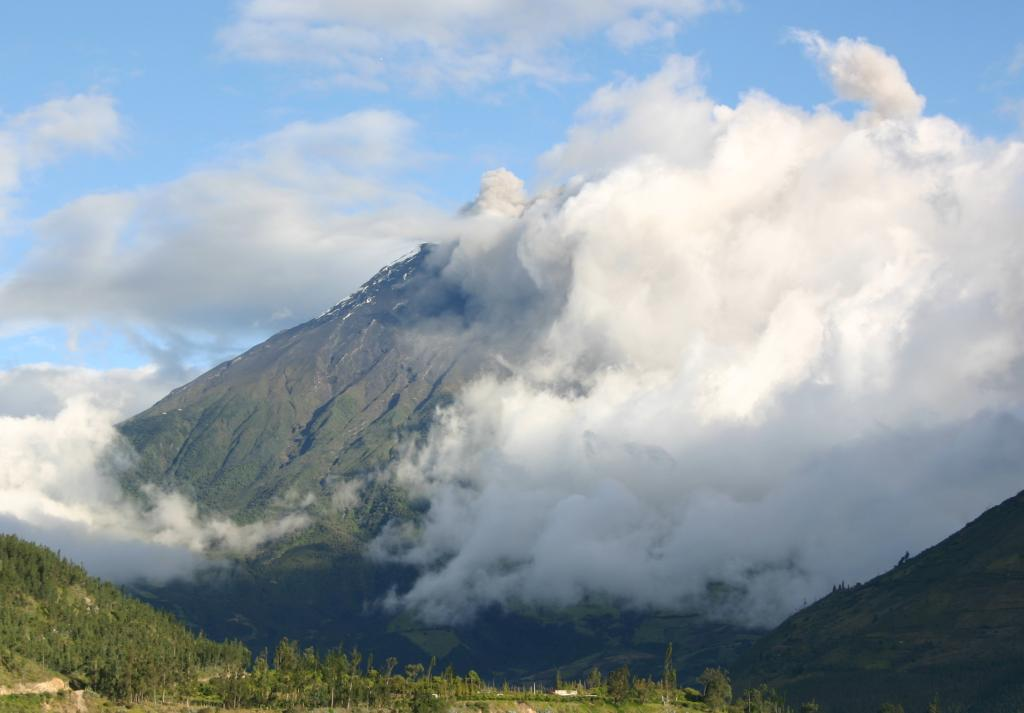
\includegraphics[width=0.9\hsize]{./figures/pics/tungurahua1.jpg}
\end{center}
\caption{\small {\bf Volc\'{a}n Tungurahua.}}
\label{fig-tungurahua}
\end{figure}

Volc\'{a}n Tungurahua (78.43$^\circ$W, 1.45$^\circ$S) is located on the
central part of the Eastern Cordillera of the Ecuadorean Andes
(Figures~\ref{fig-map}~and~\ref{fig-tungurahua}). Its current cone
has a steep flank (30-35$^\circ$ slopes) and a crater at the upper part of
its northwestern flank. Ba\~{n}os, an important tourist destination in
Ecuador with 25,000 inhabitants, is located at the foot of the volcano
close to Agoyan, one of the country's largest hydroelectric plants. Rural
communities are dispersed all around the volcano's lower flanks.

Geological studies show that Volc\'{a}n Tungurahua has produced Plinian-type
eruptions as well as at least two sector collapses ($\approx$ 13,000 
and 3,000 years b.p.~\cite{Hall99}). Since colonial times (1534), 
five eruptive cycles have occurred: 1641--1646, 1773--1781, 1886--1888,
1916--1918, and 1999--present. Generally, these eruptions were
characterized by tephra-and-ash falls covering the volcano flanks,
especially the western slopes, lahars, pyroclastic flows, and 
lava flows running down the north, west and south-western
valleys.

The current eruptive period was preceded by anomalous
seismicity first detected in 1993 by the local seismic
network~\cite{Ruiz94}.
In October 1999, after a few months of increasing
seismicity, Tungurahua emitted an ash column with incandescent blocks.
This activity led to the evacuation of more than 16,000 residents from
the surrounding areas.  As of August 2004, more than 1,900 volcanic
explosions have been recorded at Tungurahua by the Instituto Geof\'{i}sico
in Quito.  Activity has been grouped into eight eruptive cycles. The
last cycle started on May 2004 and reached its climax in June. These
eruptive periods have manifested ash emissions, and vulcanian and
strombolian activity. 

Volc\'{a}n Tungurahua is monitored by the Instituto Geof\'{i}sico of the
Escuela Politecnica Nacional (IGEPN) using a seismic network of seven
short-period stations, one broadband station, two tiltmeters, five
deformation
control lines, acoustic flow meters, and an SO$_2$-concentration
measurement system. In November 1999, a temporary microphone for
recording infrasound signals was deployed in a ridge just in front of
the volcano northwestern flank~\cite{Johnson03}.
In addition, numerous scientific campaigns, such as ours, have deployed 
temporary monitoring stations on the volcano.



\subsection{Deployment}

%My coordinate for TGUI seismometer is S01.43561, W078.46380, ELEV2889 m
%Relative to this position (0,0), my GPS tells me that:
%MOTE2 is 7 m north and 4 m east
%MOTE3 is 17 m north and 4 m west (-4 m east)
%MOTE4 is 1 m north and 2 m east

Our sensor network deployment was colocated with a wired seismic and
infrasound station used by researchers from UNC and IGEPN.  The deployment
station was located via GPS at 78.46380$^\circ$W, 1.43561$^\circ$S at
an elevation of 2889~m. 

As described previously, the aggregator node transmits data via a FreeWave
modem to a laptop acting as a base station. The laptop was kept at the 
volcano observatory operated by IGEPN, which is located 9~km away from 
the monitoring station. The observatory is in a valley with direct
line-of-sight to the monitoring station on the volcano.
A pair of 9~dBi 900~MHz Yagi antennas (Figure~\ref{fig-infrasound}(c)) were used to
establish connectivity between the two FreeWave modems. The GPS receiver
and FreeWave modem were powered by a 12~V car battery (smaller lead-acid
batteries were used for testing but are disallowed on commercial air
flights). All other nodes were powered by 2~AA batteries and operated
continuously during the 54-hour deployment.

The aggregator node, GPS receiver, FreeWave modem, Yagi antenna, and
car battery were placed at the foot of a tree. One of the infrasonic
nodes was placed about 1~m above ground in the same tree. Another node was
placed 6.3~m away in a second tree, while the third node was placed
10.7~m away on a tree stump. Infrasound nodes were elevated in trees both to
improve radio reception and to minimize molestation by cows grazing nearby.
The terrain at this location was fairly steep with a large amount of
vegetation, making it difficult to select locations further away from the
aggregator node.

% Placement of sensor nodes at Juive station
% Colocation with wired seismic and acoustic array
% Use of long-distance Yagi antenna, car batteries

\subsection{Data analysis}

\begin{figure}[t]
\begin{center}
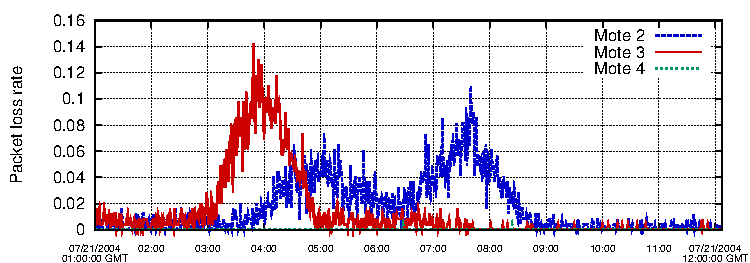
\includegraphics[width=1.0\hsize]{./figures/loss/lossrate.pdf} \\
\vspace{0.1in}
\begin{small}
\begin{tabular}{|llll|} \hline
{\em Mote} & {\em Received pkts} & {\em Lost pkts} & {\em loss rate} \\ \hline
{\em node 2} & 19470100 & 555696 & 2.77\% \\
{\em node 3} & 19039684 & 995416 & 4.96\% \\
{\em node 4} & 19584438 & 290525 & 1.46\% \\ \hline
\end{tabular}
\end{small}
\end{center}
\caption{\small {\bf Packet reception and loss statistics.}
{\em The graph shows packet loss rate, averaged over one-minute intervals,
for an 11-hour trace. Mote~4 exhibited negligible losses during this
time. The table summarizes packet loss over the
entire 54-hour deployment.}}
\label{fig-lossrate}
\end{figure}

We logged over 54~hours of continuous data from the sensor
network. Analyzing this raw data presented a number of challenges.
Although the infrasound nodes use a retransmission scheme to improve
reliability, a large number of packets are missing from the recorded
dataset. On several occasions, the FreeWave modems would experience
short dropouts of several seconds, causing data from all nodes to be
lost. In addition, GPS timestamp messages from the GPS receiver may not
have been received at the basestation, although the infrasound motes may
have received the message. Finally, on a number of occasions,
duplicate packets were recorded, most likely due to a lost acknowledgment
and redundant retransmission.  
Before registering the data to a common
timebase as described in Section~\ref{sec-regression}, it was necessary to
``clean up'' the raw logs by accounting for lost and duplicate packets.

The loss rate for each node varied during the deployment.
Figure~\ref{fig-lossrate} shows the loss rate, averaged over
one-minute intervals, for an 11-hour trace. We believe that the
gradual variation in loss is due to weather conditions (e.g., rain)
affecting radio transmission, although it is possible that temperature
fluctuations (heating and cooling of components in the Pelican cases)
may have contributed to this effect as well.
Mote~4 experienced very low loss, due 
to its positioning with a clear line-of-sight to the receiver.
Note that Mote~2, despite being located in the tree above the receiver,
experienced somewhat higher losses, probably due to antenna orientation.
Figure~\ref{fig-lossrate} summarizes the packet loss rate for each 
of the motes during the entire deployment.

% Overall statistics (total amount of data, how many eruptions)
% Statistics on lost packets, dup packets, out of order packets, over time
% Details on time regression (from Hassan's scripts)
% How much error in the regression

% Show a figure with an example explosion
% (also with Mario's seismic and acoustic data alongside)

% Look at some explosions and see if time delay between arrivals is
% consistent

\begin{figure*}[t]
\begin{center}
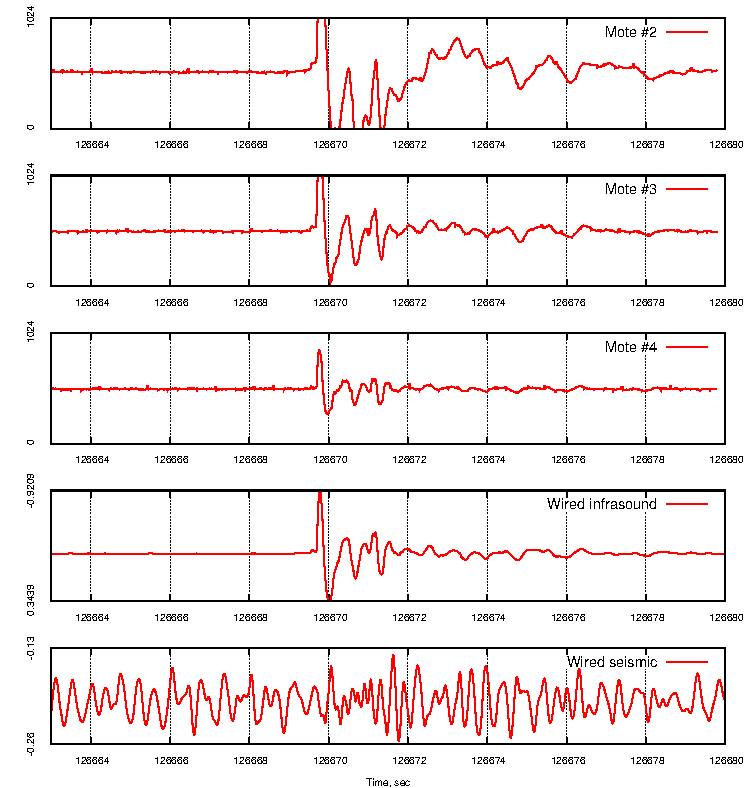
\includegraphics[width=0.7\hsize]{./figures/explosion/explosion.pdf}
\end{center}
\caption{\small {\bf Example infrasonic and seismic data from an
explosion at Tungurahua.} {\em The top three graphs show the signal
recorded by our wireless infrasonic sensor network
(July 21 2004 at 11:11:00 GMT).
The bottom two graphs show infrasonic and seismic signals from the
same explosion recorded by a colocated wired station.}}
\label{fig-explosion}
\end{figure*}

Through visual inspection of the time-regressed logs, we manually
verified well-correlated infrasonic signals from nine separate explosions 
recorded during our deployment. The frequency of explosions varied
greatly, with inter-explosion times ranging from 1~hour to over 24~hours.
Data recorded by our sensor array during an example explosion is 
shown in Figure~\ref{fig-explosion}.
Infrasonic and seismic data from the colocated wired station is shown
for comparison. As the figure shows, the wireless array demonstrates
very good correlation with wired station.
Note that the seismic signal precedes the acoustic by
several seconds due to its faster propagation speed.

